\documentclass[12pt]{article}

\newif\ifdraft\drafttrue  % set true to show comments
% \newif\ifdraft\draftfalse  % set true to show comments
\newif\ifanon\anonfalse    % set true to suppress names, etc.
\newif\ifappendices\appendicesfalse

%\PassOptionsToPackage{usenames,dvipsnames,svgnames,table}{xcolor}

\usepackage[usenames,dvipsnames,svgnames,table]{xcolor}
\usepackage{amsmath}
\usepackage[capitalise]{cleveref}
\usepackage{makecell}%To keep spacing of text in tables
\usepackage{nccmath}
\usepackage{mathtools}
\usepackage{bussproofs}
\usepackage{varwidth}
\usepackage{amsthm}
\usepackage{csvsimple}
\usepackage{thmtools,thm-restate}
\usepackage{changepage}
\usepackage{booktabs}
\usepackage{amssymb}
\usepackage{enumitem}
\usepackage{multirow,bigdelim}
\usepackage{multicol}
\usepackage{siunitx}
\usepackage{listings}
\usepackage{letltxmacro}
\usepackage{sansmath}
\usepackage{url}
\usepackage{flushend}
\usepackage{microtype}
\usepackage[utf8]{inputenc}
\usepackage{mathpartir}
\usepackage{empheq}
\usepackage{array}
\usepackage{pgfplots}
\usepackage{stmaryrd}
\usepackage{courier}
\usepackage{qtree}
\usepackage[normalem]{ulem}
\usepackage{relsize}
\usepackage{tikz}
\usepackage{algorithm}
\usepackage[noend]{algpseudocode}
\usepackage{graphicx}
\usepackage{subcaption}
\usepackage{textcomp}
\usepackage{tabularx}
\usepackage{stackengine}
\usepackage{caption}
\usepackage{wrapfig}
\usepackage{remreset}
\usepackage{tabulary}
\usepackage{xspace}
\usepackage{bbm}
\usepackage{fullpage}
\usepackage[explicit]{titlesec}

% \renewcommand*\thesection{\arabic{section}.0}
% \renewcommand*\thesubsection{\arabic{section}.\arabic{subsection}}


\newtheorem*{theorem*}{Theorem}
\newenvironment{centermath}
 {\begin{center}$\displaystyle}
 {$\end{center}}
\setcellgapes{4pt}%parameter for the spacing

\lstset{ language=Caml, basicstyle=\upshape\sffamily,
keywordstyle=\upshape\sffamily\color{dkpurple}, keepspaces=true,
framexleftmargin=1ex, framexrightmargin=1ex, showstringspaces=true,
commentstyle=\itshape\rmfamily,
emph={rep,iterate,synth,collapse,perm,squash,normalize,using,ins,del,lens,let,get,put,rquot,lquot,id,swap,concat,or,disconnect,merge_left,merge_right,const},
emphstyle=\upshape\sffamily\color{dkpurple}, 
columns=fullflexible,
mathescape, 
xleftmargin=1.5em,
% BCP: I find this distracting:
stringstyle=\sffamily\color{dkblue},
}
\makeatletter
     \let\lst@oldvisiblespace\lst@visiblespace
     \def\lst@visiblespace{\,\lst@oldvisiblespace\,}
\makeatother

\setlength{\belowdisplayskip}{0pt} \setlength{\belowdisplayshortskip}{0pt}
\setlength{\abovedisplayskip}{0pt} \setlength{\abovedisplayshortskip}{0pt}

\usetikzlibrary{
  er,
  matrix,
  shapes,
  arrows,
  positioning,
  fit,
  calc,
  pgfplots.groupplots,
  arrows.meta
}
\tikzset{>={Latex}}

%%%% Hyperlinks – must come late!
%\usepackage[pdftex,%
%            pdfpagelabels,%
%            linkcolor=blue,%
%            citecolor=blue,%
%            filecolor=blue,%
%            urlcolor=blue]
%           {hyperref}

% Colors
\definecolor{dkblue}{rgb}{0,0.1,0.5}
\definecolor{dkgreen}{rgb}{0,0.6,0}
\definecolor{dkred}{rgb}{0.6,0,0}
\definecolor{dkpurple}{rgb}{0.4,0,0.6}
\definecolor{olive}{rgb}{0.4, 0.4, 0.0}
\definecolor{teal}{rgb}{0.0,0.5,0.5}
\definecolor{orange}{rgb}{0.9,0.6,0.2}
\definecolor{lightyellow}{RGB}{255, 255, 179}
\definecolor{lightgreen}{RGB}{170, 255, 220}
\definecolor{teal}{RGB}{141,211,199}
\definecolor{darkbrown}{RGB}{121,37,0}

% remove whitespace before and after multicols
\setlength{\multicolsep}{0pt}

% renewtheorem https://tex.stackexchange.com/questions/103013/is-there-a-renewtheorem-equivalent-of-renewcommand-using-amsthm-and-not-ntheo
\makeatletter
\def\renewtheorem#1{%
  \expandafter\let\csname#1\endcsname\relax
  \expandafter\let\csname c@#1\endcsname\relax
  \gdef\renewtheorem@envname{#1}
  \renewtheorem@secpar
}
\def\renewtheorem@secpar{\@ifnextchar[{\renewtheorem@numberedlike}{\renewtheorem@nonumberedlike}}
\def\renewtheorem@numberedlike[#1]#2{\newtheorem{\renewtheorem@envname}[#1]{#2}}
\def\renewtheorem@nonumberedlike#1{  
\def\renewtheorem@caption{#1}
\edef\renewtheorem@nowithin{\noexpand\newtheorem{\renewtheorem@envname}{\renewtheorem@caption}}
\renewtheorem@thirdpar
}
\def\renewtheorem@thirdpar{\@ifnextchar[{\renewtheorem@within}{\renewtheorem@nowithin}}
\def\renewtheorem@within[#1]{\renewtheorem@nowithin[#1]}
\makeatother

\pgfplotsset{
% override style for non-boxed plots
    % which is the case for both sub-plots
    every non boxed x axis/.style={} 
}

\newenvironment{mathprooftree}
  {\varwidth{.9\textwidth}\centering\leavevmode}
  {\DisplayProof\endvarwidth}

\newcommand{\FINISH}[3]{\ifdraft\textcolor{#1}{[#2: #3]}\fi}
\newcommand{\bcp}[1]{\FINISH{dkred}{B}{#1}}
\newcommand{\BCP}[1]{\FINISH{dkred}{B}{\bf #1}}
\newcommand{\afm}[1]{\FINISH{dkgreen}{A}{#1}}
\newcommand{\dpw}[1]{\FINISH{dkblue}{D}{#1}}
\newcommand{\saz}[1]{\FINISH{orange}{S}{#1}}
\newcommand{\ksf}[1]{\FINISH{teal}{K}{#1}}
\newcommand{\revised}[1]{\FINISH{dkred}{#1}}

\newcommand{\IE}{\emph{i.e.}}
\newcommand{\EG}{\emph{e.g.}}
\newcommand{\ETC}{\emph{etc.}}

\theoremstyle{definition}
\renewtheorem{theorem}{Theorem}
\newtheorem{mylemma}{Lemma}
\renewtheorem{corollary}{Corollary}
\renewtheorem{conjecture}{Conjecture}
\renewtheorem{definition}{Definition}
\newtheorem{property}{Property}
\theoremstyle{plain}
\theoremstyle{remark}
\newtheorem{subcase}{Subcase}
\theoremstyle{remark}
\newtheorem{case}{Case}
\makeatletter
\@addtoreset{subcase}{case}
\@addtoreset{case}{mylemma}
\@addtoreset{case}{theorem}
\@addtoreset{case}{corollary}
\@addtoreset{case}{definition}
\@addtoreset{case}{definition}
\@removefromreset{theorem}{section}
\makeatother

\algnewcommand\algorithmicswitch{\textbf{switch}}
\algnewcommand\algorithmicmatch{\textbf{match}}
\algnewcommand\algorithmiccase{\textbf{case}}
\algnewcommand\algorithmicwith{\textbf{with}}
\algnewcommand\algorithmicforeach{\textbf{foreach}}
\algnewcommand\Assert[1]{\State \algorithmicassert(#1)}%
% New "environments"
\algdef{SE}[SWITCH]{Switch}{EndSwitch}[1]{\algorithmicmatch\ #1\ \algorithmicwith}{\algorithmicend\ \algorithmicswitch}%
\algdef{SE}[CASE]{Case}{EndCase}[1]{$|~$ #1 $\rightarrow$}{\algorithmicend\ \algorithmiccase}%
\algdef{SE}[FOREACH]{ForEach}{EndForEach}[2]{\algorithmicforeach\ #1 $\in$ #2}{\algorithmicend\ \algorithmicforeach}%
\algdef{SE}[CaseTwo]{CaseTwo}{EndCaseTwo}[2]{$|~$ #1 $\rightarrow$ #2}{\algorithmicend\ \algorithmiccase}%
\algtext*{EndSwitch}%
\algtext*{EndCase}%
\algtext*{EndCaseTwo}%
\algtext*{EndSecondCase}%
\algtext*{EndForEach}%



\newcommand{\CF}[1]{\ensuremath{\mathsf{#1}}}         % Code Font
\newcommand{\SmallCF}[1]{{\small \mathsf{#1}}}
\newcommand{\PCF}[1]{\textproc{#1}}
\newcommand{\VarCF}[1]{{\color{darkbrown} \CF{#1}}}
\newcommand{\StringCF}[1]{\CF{\textcolor{blue}{#1}}}
\newcommand{\KW}[1]{\CF{\textcolor{dkpurple}{#1}}}
\newcommand{\Regex}{\ensuremath{\mathit{S}}\xspace}         % Regular Expression
\newcommand{\RegexType}{\ensuremath{\textit{Regex}}}
\newcommand{\EquivRegexType}{\ensuremath{\textit{Regex}/\sim}}
\newcommand{\BooleanAnd}{\ensuremath{~\wedge~}}
\newcommand{\BooleanOr}{\ensuremath{\vee}}
\newcommand{\BooleanImplies}{\ensuremath{\Rightarrow}}
\newcommand{\Rewrite}{\ensuremath{\rightarrow}}
\newcommand{\RewriteAtom}{\ensuremath{\Rewrite_\Atom}}
\newcommand{\RewriteDNF}{\ensuremath{\Rewrite_\DNFRegex}}
\newcommand{\ConcatDNF}{\ensuremath{\odot}}
\newcommand{\ConcatDNFOf}[2]{\ensuremath{#1\ConcatDNF#2}}
\newcommand{\BigConcatDNF}{\ensuremath{\bigodot}}
\newcommand{\ConcatSequence}{\ensuremath{\odot_{\Sequence}}}
\newcommand{\ConcatSequenceOf}[2]{\ensuremath{#1\ConcatSequence#2}}
\newcommand{\ConcatPermutation}{\ensuremath{\odot}}
\newcommand{\ConcatPermutationOf}[2]{\ensuremath{#1\ConcatPermutation#2}}
\newcommand{\SwapPermutation}{\ensuremath{\circledS}}
\newcommand{\SwapPermutationOf}[2]{\ensuremath{#1\SwapPermutation#2}}
\newcommand{\DistributePermutation}{\ensuremath{\otimes}}
\newcommand{\DistributePermutationOf}[2]{\ensuremath{#1\DistributePermutation#2}}
\newcommand{\DistributeSwapPermutation}{\ensuremath{\otimes^{\mathit{s}}}}
\newcommand{\DistributeSwapPermutationOf}[2]{\ensuremath{#1\DistributeSwapPermutation#2}}
\newcommand{\ConcatSequenceLens}{\ensuremath{\odot_{\SequenceLens}}}
\newcommand{\ConcatSequenceLensOf}[2]{\ensuremath{#1\ConcatSequenceLens#2}}
\newcommand{\ConcatDNFLens}{\ensuremath{\odot}}
\newcommand{\ConcatDNFLensOf}[2]{\ensuremath{#1\ConcatDNFLens#2}}
\newcommand{\SwapSequenceLens}{\ensuremath{\circledS_{\SequenceLens}}}
\newcommand{\SwapSequenceLensOf}[2]{\ensuremath{#1\SwapSequenceLens#2}}
\newcommand{\SwapDNFLens}{\ensuremath{\circledS}}
\newcommand{\SwapDNFLensOf}[2]{\ensuremath{#1\SwapDNFLens#2}}
\newcommand{\RepeatDNFOfTimes}[1]{\ensuremath{^{#1}}}
\newcommand{\RepeatDNFOf}[2]{\ensuremath{{#2}\RepeatDNFOfTimes{#1}}}
\newcommand{\RepeatDNFLensOfTimes}[1]{\ensuremath{^{#1}}}
\newcommand{\RepeatDNFLensOf}[2]{\ensuremath{{#2}\RepeatDNFLensOfTimes{#1}}}
\newcommand{\OrDNF}{\ensuremath{\oplus}}
\newcommand{\OrDNFOf}[3]{\ensuremath{#1\OrDNF_{#3}#2}}
\newcommand{\OrDNFLens}{\ensuremath{\oplus}}
\newcommand{\OrDNFLensOf}[2]{\ensuremath{#1\OrDNFLens#2}}
\newcommand{\PutRSym}{\ensuremath{\mathit{putr}}}
\newcommand{\PutLSym}{\ensuremath{\mathit{putl}}}
\newcommand{\PutRSymOf}[1]{\ensuremath{\PutRSym \App #1}}
\newcommand{\PutLSymOf}[1]{\ensuremath{\PutLSym \App #1}}
\newcommand{\RegexAlt}{\ensuremath{\mathit{T}}\xspace}         % Regular Expression
\newcommand{\RegexAltAlt}{\ensuremath{\mathit{U}}\xspace}         % Regular Expression
\newcommand{\Or}{\ensuremath{~|~}}
\newcommand{\RegexOr}[2]{\ensuremath{#1\Or#2}}
\newcommand{\SubN}{\textsubscript{n}}
\newcommand{\RegexConcat}[2]{\ensuremath{#1\cdot#2}}
\newcommand{\EmptyString}{\ensuremath{\epsilon}}
\newcommand{\StringConcat}[2]{\ensuremath{#1\cdot#2}}
\newcommand{\HasSemantics}{\ensuremath{\triangleright}}
\newcommand{\DerivesLens}{\ensuremath{\vdash}}
\newcommand{\DerivesDNFLens}{\ensuremath{\vdash_{\DNFLens}}}
\newcommand{\DerivesSequenceLens}{\ensuremath{\vdash_{\SequenceLens}}}
\newcommand{\DerivesAtomLens}{\ensuremath{\vdash_{\AtomLens}}}
\newcommand{\DerivesStringRegex}{\ensuremath{\vdash}}
\newcommand{\DerivesAtomRewrite}{\ensuremath{\vdash}}
\newcommand{\DerivesDNFRewrite}{\ensuremath{\vdash}}
\newcommand{\Concat}{\ensuremath{\cdot}}
\newcommand{\Union}{\ensuremath{\cup}}
\newcommand{\Intersect}{\ensuremath{\cap}}
\newcommand{\BigUnion}{\ensuremath{\bigcup}}
\newcommand{\BigIntersect}{\ensuremath{\bigcap}}
\newcommand{\denot}[1]{\ensuremath{[ \! [#1] \! ]}}
\newcommand{\SemanticsOf}[1]{\ensuremath{[ \! [#1] \! ]}}
\newcommand{\SetOf}[1]{\ensuremath{\{#1\}}}
\newcommand{\RegexVariable}{\ensuremath{\mathit{U}}}   % User Defined
\newcommand{\RegexVariableAlt}{\ensuremath{\mathit{V}}}
\newcommand{\LensVariable}{\ensuremath{\mathit{L}}}
\newcommand{\ExampledRegex}{\ensuremath{\mathit{er}}} % Exampled Regex
\newcommand{\UnambigItOf}[1]{\ensuremath{#1^{*!}}}
\newcommand{\UnambigConcat}{\ensuremath{\Concat^!}}
\newcommand{\SequenceUnambigConcatOf}[1]{\ensuremath{\UnambigConcat(#1)}}
\newcommand{\UnambigConcatOf}[2]{\ensuremath{#1 \UnambigConcat #2}}
\newcommand{\UnambigOrOf}[2]{\ensuremath{\LanguageOf{#1} \cap \LanguageOf{#2} = \emptyset}}
\newcommand{\Atom}{\ensuremath{\mathit{A}}}          % Atoms
\newcommand{\AtomAlt}{\ensuremath{\mathit{B}}}
\newcommand{\AtomType}{\ensuremath{\mathit{Atom}}}
\newcommand{\App}{\ensuremath{\,}}
\newcommand{\Sequence}{\ensuremath{\mathit{SQ}}}
\newcommand{\SequenceType}{\ensuremath{\mathit{Sequence}}}
\newcommand{\LetIn}[2]{\ensuremath{\text{let } #1 = #2\text{ in }}}
\newcommand{\LetWhereIn}[3]{\ensuremath{\text{let } #1 = #2 \text{ where } #3 \text{ in }}}
\newcommand{\Where}{\ensuremath{\text{ where }}}
\newcommand{\ClauseAlt}{\ensuremath{\mathit{bl}}}       % Clauses
\newcommand{\SequenceAlt}{\ensuremath{\mathit{TQ}}}
\newcommand{\DNFRegex}{\ensuremath{\mathit{DS}}}         % Regular Expression
\newcommand{\DNFRegexAlt}{\ensuremath{\mathit{DT}}}    %Alt Regex
\newcommand{\DNFRegexType}{\ensuremath{\mathit{DNF}}}
\newcommand{\LensContext}{\ensuremath{\Gamma}}
\newcommand{\RegexContext}{\ensuremath{\Delta}}  % Context
\newcommand{\FullContext}{\ensuremath{\Delta, \Gamma}}
\newcommand{\String}{\ensuremath{\mathit{s}}\xspace}        % String
\newcommand{\StringAlt}{\ensuremath{\mathit{t}}}        % StringAlt
\newcommand{\StringAltAlt}{\ensuremath{\mathit{u}}}        % StringAltAlt
\newcommand{\ExampleNumberList}{\ensuremath{\mathit{enl}}} %Example Number List
\newcommand{\ExampleNumberListList}{\ensuremath{\mathit{enll}}}
\newcommand{\ExampleStringList}{\ensuremath{\mathit{esl}}}
\newcommand{\StringList}{\ensuremath{\mathit{sl}}}
\newcommand{\Natural}{\ensuremath{\mathit{n}}}
\newcommand{\Interleaving}[1]{\ensuremath{\mathit{interleaving}(#1)}}
\newcommand{\Interleave}{\ensuremath{\mathit{interleave}}}
\newcommand{\BinaryInterleave}[2]{\ensuremath{\mathit{interleave}(#1,#2)}}
\newcommand{\NAryInterleave}[2]{\ensuremath{\mathit{interleave}(#1,\ldots,#2)}}
\newcommand{\Combine}{\ensuremath{\mathit{combine}}}
\newcommand{\List}{\ensuremath{\mathit{l}}}
\newcommand{\ValidCombine}[2]{\ensuremath{\mathit{validcombine}(#1,#2)}}
\newcommand{\ValidRegexContext}[2]{\ensuremath{\mathit{validregexcontext}(#1,#2)}}
\newcommand{\Parent}[1]{\ensuremath{\mathit{parent}(#1)}}
\newcommand{\Parented}[1]{\ensuremath{mathit{parented}(#1)}}
\newcommand{\CombineString}[1]{\ensuremath{\mathit{combine}_{\ExampleStringList}(#1)}}
\newcommand{\CombineList}[1]{\ensuremath{\mathit{combine}_{\ExampleNumberListList}(#1)}}
\newcommand{\Length}[1]{\ensuremath{\mathit{len}(#1)}}
\newcommand{\Language}{\ensuremath{L}}
\newcommand{\LanguageOf}[1]{\ensuremath{\mathcal{L}(#1)}}
\newcommand{\LanguageUnderContextOf}[2]{\ensuremath{\Language{}_{#1}(#2)}}
\newcommand{\ParseTree}{\ensuremath{\mathit{p}}}
\newcommand{\ParseTreeAlt}{\ensuremath{\mathit{q}}}
\newcommand{\ParseTrees}{\ensuremath{\mathit{ps}}}
\newcommand{\ParseTreeAlts}{\ensuremath{\mathit{qs}}}
\newcommand{\StarParse}[1]{\ensuremath{\mathit{starparse}(#1)}}
\newcommand{\LeftChoiceParse}[1]{\ensuremath{\mathit{l}.(#1)}}
\newcommand{\RightChoiceParse}[1]{\ensuremath{\mathit{r}.(#1)}}
\newcommand{\RangeExcInc}[2]{\ensuremath{(#1,#2]}}
\newcommand{\RangeIncInc}[2]{\ensuremath{[#1,#2]}}

\newcommand{\Lens}{\ensuremath{\mathit{\ell}}\xspace}
\newcommand{\AtomLens}{\ensuremath{\mathit{al}}}
\newcommand{\IterateAtomType}{\textit{Iterate}}
\newcommand{\ConcatedAtomsLens}{\ensuremath{\mathit{cal}}}
\newcommand{\OredClausesLens}{\ensuremath{\mathit{ocl}}}
\newcommand{\ClauseLens}{\ensuremath{\mathit{cll}}}
\newcommand{\SequenceLens}{\ensuremath{\mathit{sql}}}
\newcommand{\SequenceLensType}{\ensuremath{\mathit{SequenceLens}}}
\newcommand{\DNFLens}{\ensuremath{\mathit{dl}}}
\newcommand{\DNFLensType}{\ensuremath{\mathit{DNFLens}}}
\newcommand{\AtomLensType}{\ensuremath{\mathit{AtomLens}}}
\newcommand{\SynSim}[2]{\ensuremath{#1 \sim_{\mathit{sym}} #2}}
\newcommand{\ExdSynSim}[3]{\ensuremath{#2 \sim_{\mathit{sym},#1} #3}}

\newcommand{\PermutationSetOf}[1]{\ensuremath{S_{#1}}}
\newcommand{\Permutation}{\ensuremath{\sigma}}

\newcommand{\Star}{\ensuremath{^*}}
\newcommand{\StarOf}[1]{\ensuremath{{#1}\Star}}
\newcommand{\ConstLens}{\ensuremath{\mathit{const}}}
\newcommand{\ConstLensOf}[2]{\ensuremath{\ConstLens(#1,#2)}}
\newcommand{\ConcatLens}{\ensuremath{\KW{concat}}}
\newcommand{\ConcatLensOf}[2]{\ensuremath{\ConcatLens(#1,#2)}}
\newcommand{\ConcatLensShortOf}[2]{\ensuremath{\mathit{c}(#1,#2)}}
\newcommand{\SwapLens}{\ensuremath{\KW{swap}}\xspace}
\newcommand{\SwapLensOf}[2]{\ensuremath{\SwapLens(#1,#2)}}
\newcommand{\SwapLensShortOf}[2]{\ensuremath{\mathit{s}(#1,#2)}}
\newcommand{\OrLens}{\ensuremath{\KW{or}}\xspace}
\newcommand{\OrLensOf}[2]{\ensuremath{\OrLens(#1,#2)}}
\newcommand{\IdentityLens}{\ensuremath{\KW{id}}}
\newcommand{\IdentityLensOf}[1]{\ensuremath{\IdentityLens(#1)}}
\newcommand{\IdentityLensShortT}{\ensuremath{\mathit{id}}}
\newcommand{\IdentityLensShortOf}[1]{\ensuremath{\IdentityLensShortT_{#1}}}
\newcommand{\IterateLens}{\ensuremath{\KW{iterate}}\xspace}
\newcommand{\IterateLensOf}[1]{\ensuremath{\mathit{\IterateLens(#1)}}}
\newcommand{\Identity}{\ensuremath{\mathit{id}}}
\newcommand{\Compose}{\ensuremath{\circ}}
\newcommand{\ComposeLensOf}[2]{\ensuremath{#1\mathrel{;}#2}}
\newcommand{\Disconnect}{\ensuremath{\KW{disc}}\xspace}
\newcommand{\DisconnectOf}[4]{\ensuremath{\Disconnect(#1,#2,#3,#4)}}
\newcommand{\MergeL}{\ensuremath{\KW{merge\_left}}\xspace}
\newcommand{\MergeLOf}[2]{\ensuremath{\MergeL(#1,#2)}}
\newcommand{\MergeR}{\ensuremath{\KW{merge\_right}}\xspace}
\newcommand{\MergeROf}[2]{\ensuremath{\MergeR(#1,#2)}}
\newcommand{\Invert}{\ensuremath{\KW{invert}}}
\newcommand{\InvertOf}[1]{\ensuremath{\Invert(#1)}}

% GRAMMAR OPERATORS
\newcommand{\GBar}{\ensuremath{~|~}}
\newcommand{\GIndent}{\hspace{.5in}}
\newcommand{\GEq}{\ensuremath{::=~}}
\newcommand{\GEmp}{\ensuremath{\cdot}}
\newcommand{\Perm}{\ensuremath{\mathit{Perm}}}
\newcommand{\Nats}{\ensuremath{\mathbb{N}}}

\newcommand{\InverseOf}[1]{\ensuremath{#1^{-1}}}
\newcommand{\FloorOf}[1]{\ensuremath{\lfloor#1\rfloor}}
\newcommand{\CeilOf}[1]{\ensuremath{\lceil#1\rceil}}
\newcommand{\OfType}{\ensuremath{:}}
\newcommand{\OfRewritelessType}{\ensuremath{\,\,\tilde{\OfType}\,\,}}
\newcommand{\MapsBetweenTypeOf}[2]{\ensuremath{#1 \Leftrightarrow #2}}
\newcommand{\ArrowTypeOf}[2]{\ensuremath{#1 \rightarrow #2}}
\newcommand{\SizeOf}[1]{\ensuremath{|#1|}}

\newcommand{\ToDNFRegex}{\ensuremath{\Downarrow}}
\newcommand{\ToDNFRegexOf}[1]{\ensuremath{\ToDNFRegex\mkern-4mu #1}}
\newcommand{\ToRegex}{\ensuremath{\Uparrow}}
\newcommand{\ToRegexOf}[1]{\ensuremath{\ToRegex\mkern-4mu #1}}

\newcommand{\SuchThat}{\ensuremath{~|~}}
\newcommand{\That}{\ensuremath{~.~}}
\newcommand{\Given}{\ensuremath{~|~}}

\newcommand{\LeftQuotientOf}[2]{\ensuremath{#1\backslash#2}}
\newcommand{\RightQuotientOf}[2]{\ensuremath{#1\slash#2}}

\newcommand{\SuffixOf}[1]{\ensuremath{S_{#1}}}
\newcommand{\PrefixOf}[1]{\ensuremath{P_{#1}}}

\newcommand{\ComplementOf}[1]{\ensuremath{\bar{#1}}}

\newcommand{\Alphabet}{\ensuremath{\Sigma}}
\newcommand{\Character}{\ensuremath{c}}
\newcommand{\CharacterAlt}{\ensuremath{d}}

\newcommand{\SequenceLeft}{\ensuremath{[}}
\newcommand{\SequenceRight}{\ensuremath{]}}
\newcommand{\SequenceOf}[1]{\ensuremath{\SequenceLeft#1\SequenceRight}}
\newcommand{\SeqSep}{\ensuremath{\mkern-1mu\Concat\mkern-1mu}}
\newcommand{\DNFLeft}{\ensuremath{\langle}}
\newcommand{\DNFRight}{\ensuremath{\rangle}}
\newcommand{\DNFOf}[1]{\ensuremath{\DNFLeft#1\DNFRight}}
\newcommand{\DNFSep}{\ensuremath{\Or}}
\newcommand{\SequenceLensLeft}{\ensuremath{[}}
\newcommand{\SequenceLensRight}{\ensuremath{]}}
\newcommand{\SequenceLensOf}[1]{\ensuremath{\SequenceLensLeft#1\SequenceLensRight}}
\newcommand{\SeqLSep}{\ensuremath{\mkern-1mu\Concat\mkern-1mu}}
\newcommand{\DNFLensLeft}{\ensuremath{\langle}}
\newcommand{\DNFLensRight}{\ensuremath{\rangle}}
\newcommand{\DNFLensOf}[1]{\ensuremath{\DNFLensLeft#1\DNFLensRight}}
\newcommand{\DNFLSep}{\ensuremath{\Or}}


\newcommand{\ConstantLensRule}{\textsc{Constant Lens}}
\newcommand{\IdentityLensRule}{\textsc{Identity Lens}}
\newcommand{\IterateLensRule}{\textsc{Iterate Lens}}
\newcommand{\ConcatLensRule}{\textsc{Concat Lens}}
\newcommand{\SwapLensRule}{\textsc{Swap Lens}}
\newcommand{\OrLensRule}{\textsc{Or Lens}}
\newcommand{\ComposeLensRule}{\textsc{Compose Lens}}
\newcommand{\RewriteRegexLensRule}{\textsc{Rewrite Regex Lens}}

\newcommand{\AtomUnrollstarLeftRule}{\textsc{Atom Unrollstar\SubLeft}}
\newcommand{\AtomUnrollstarRightRule}{\textsc{Atom Unrollstar\SubRight}}
\newcommand{\ParallelAtomStructuralRewriteRule}{\textsc{Parallel Atom Structural Rewrite}}
\newcommand{\ParallelSwapAtomStructuralRewriteRule}{\textsc{Parallel Swap Atom Structural Rewrite}}
\newcommand{\AtomStructuralRewriteRule}{\textsc{Atom Structural Rewrite}}
\newcommand{\DNFStructuralRewriteRule}{\textsc{DNF Structural Rewrite}}
\newcommand{\ParallelDNFStructuralRewriteRule}{\textsc{Parallel DNF Structural Rewrite}}
\newcommand{\ParallelSwapDNFStructuralRewriteRule}{\textsc{Parallel Swap DNF Structural Rewrite}}
\newcommand{\IdentityRewriteRule}{\textsc{Identity Rewrite}}
\newcommand{\DNFReorderRule}{\textsc{DNF Reorder}}

\newcommand{\SequenceLensRule}{\textsc{Sequence Lens}}
\newcommand{\AtomLensRule}{\textsc{Atom Lens}}
\newcommand{\DNFLensRule}{\textsc{DNF Lens}}
\newcommand{\RewriteDNFRegexLensRule}{\textsc{Rewrite DNF Regex Lens}}

\newcommand{\SubLeft}{\textsubscript{L}}
\newcommand{\SubRight}{\textsubscript{R}}

\newcommand{\Set}{\ensuremath{\mathit{S}}}

\newcommand{\OrIdentityRule}{\textit{+ Ident}}
\newcommand{\EmptyProjectionRightRule}{\textit{0 Proj\SubRight{}}}
\newcommand{\EmptyProjectionLeftRule}{\textit{0 Proj\SubLeft{}}}
\newcommand{\ConcatAssocRule}{\textit{\Concat{} Assoc}}
\newcommand{\OrAssociativityRule}{\textit{\Or{} Assoc}}
\newcommand{\OrCommutativityRule}{\textit{\Or{} Comm}}
\newcommand{\DistributivityLeftRule}{\textit{Dist\SubRight{}}}
\newcommand{\DistributivityRightRule}{\textit{Dist\SubLeft{}}}
\newcommand{\ConcatIdentityLeftRule}{\textit{\Concat{} Ident\SubLeft{}}}
\newcommand{\ConcatIdentityRightRule}{\textit{\Concat{} Ident\SubRight{}}}
\newcommand{\SumstarRule}{\textit{Sumstar}}
\newcommand{\ProductstarRule}{\textit{Prodstar}}
\newcommand{\UnrollstarLeftRule}{\textit{Unrollstar\SubLeft{}}}
\newcommand{\UnrollstarRightRule}{\textit{Unrollstar\SubRight{}}}
\newcommand{\StarstarRule}{\textit{Starstar}}
\newcommand{\DicyclicityRule}{\textit{Dicyc}}
\newcommand{\Derivation}{\ensuremath{\mathcal{D}}}

\newcolumntype{q}{>{$}l<{$}}
\newcolumntype{v}{>{$}r<{$}}

\renewcommand{\subsubsection}[1]{\paragraph{{#1}}}

\newcommand{\Examples}{\ensuremath{\mathit{exs}}}

\newcommand{\ParallelReduction}{\ensuremath{\rightarrow}}
\newcommand{\ParallelRewrite}{\ensuremath{\,\mathrlap{\to}\,{\scriptstyle\parallel}\,\,\,}}
\newcommand{\ParallelRewriteAtom}{\ensuremath{\ParallelRewrite_{\Atom}}}
\newcommand{\ParallelRewriteSwap}{\ensuremath{\ParallelRewrite^{\mathit{swap}}}}
\newcommand{\ParallelRewriteSwapAtom}{\ensuremath{\ParallelRewrite^{\mathit{swap}}_{\Atom}}}

\newcommand{\Property}{\ensuremath{\mathit{p}}}
\newcommand{\Propagator}{\ensuremath{\mathit{q}}}

\newcommand{\Relation}{\ensuremath{\mathit{R}}}
\newcommand{\RelationSet}{\ensuremath{\mathit{RS}}}

\newcommand{\DiamondProperty}{\ensuremath{\mathit{confluent}}}
\newcommand{\DiamondPropertyWithPropertyOf}[1]{\ensuremath{\DiamondProperty_{#1}}}
\newcommand{\IsConfluentWithPropertyOf}[2]
    {\ensuremath{\DiamondPropertyWithPropertyOf{#2}(#1)}}
\newcommand{\BisimilarProperty}{\ensuremath{\mathit{bisimilar}}}
\newcommand{\BisimilarPropertyWithPropertyOf}[1]{\ensuremath{\BisimilarProperty_{#1}}}
\newcommand{\IsBisimilarWithPropertyOf}[2]
    {\ensuremath{\BisimilarPropertyWithPropertyOf{#2}(#1)}}

\newcommand{\Reduces}{\ensuremath{\rightarrow}}

\newcommand{\SortaEquiv}{\ensuremath{\equiv_{sorta}}}

\newcommand{\AtomEquiv}{\ensuremath{\equiv_{\Atom}}}

\newcommand{\Sep}{\ensuremath{\$}}

\newcommand{\Cross}{\ensuremath{\times}}

\newcommand{\Distance}{\ensuremath{\mathit{d}}}

\newcommand{\AbsOf}[1]{\ensuremath{|#1|}}
\newcommand{\Size}{\ensuremath{\mathit{size}}}
\newcommand{\Module}{\ensuremath{\mathit{M}}}
\newcommand{\VectorSpace}{\ensuremath{\mathit{V}}}

\newcommand{\GetDist}{\ensuremath{\mathit{dist}}}
\newcommand{\LOneNorm}{\ensuremath{\ell_1}}

\newcommand{\Sorting}{\ensuremath{\mathit{sorting}}}
\newcommand{\SortingOf}[2]{\ensuremath{\Sorting(#1,#2)}}

\newcommand{\Sort}{\ensuremath{\mathit{sort}}}
\newcommand{\SortOf}[2]{\ensuremath{\Sort(#1,#2)}}

\newcommand{\ListType}{\ensuremath{\mathit{List}}}
\newcommand{\ListTypeOf}[1]{\ensuremath{#1\,\ListType}}
\newcommand{\ListLeft}{\ensuremath{[}}
\newcommand{\ListRight}{\ensuremath{]}}
\newcommand{\ListOf}[1]{\ensuremath{\ListLeft #1 \ListRight}}
\newcommand{\DNFLeq}{\ensuremath{\leq_{DNF}}}
\newcommand{\SequenceLeq}{\ensuremath{\leq_{Seq}}}
\newcommand{\AtomLeq}{\ensuremath{\leq_{Atom}}}
\newcommand{\ILSLeq}{\ensuremath{\leq_{\mathit{intlistset}}}}
\newcommand{\ExampledDNFLeq}{\ensuremath{\leq_{DNF}^{\Examples}}}
\newcommand{\ExampledSequenceLeq}{\ensuremath{\leq_{Seq}^{\Examples}}}
\newcommand{\ExampledAtomLeq}{\ensuremath{\leq_{Atom}^{\Examples}}}
\newcommand{\DNFEq}{\ensuremath{=_{DNF}}}
\newcommand{\SequenceEq}{\ensuremath{=_{Seq}}}
\newcommand{\AtomEq}{\ensuremath{=_{Atom}}}

\newcommand{\NormalizedDNFOf}[1]{\ensuremath{\DNFOf{#1}_n}}
\newcommand{\NormalizedSequenceOf}[1]{\ensuremath{\SequenceOf{#1}_n}}
\newcommand{\NormalizedStarOf}[1]{\ensuremath{\NormalizedStarOf{#1}_n}}

\newcommand{\AtomNormalizer}{\ensuremath{\mathit{AN}}}
\newcommand{\AtomNormalizerType}{\textit{Atom Normalizer}}
\newcommand{\SequenceNormalizer}{\ensuremath{\mathit{SNN}}}
\newcommand{\SequenceNormalizerType}{\textit{Sequence Normalizer}}
\newcommand{\DNFRegexNormalizer}{\ensuremath{\mathit{DNFN}}}
\newcommand{\DNFRegexNormalizerType}{\textit{DNF Normalizer}}

\newcommand{\Normalize}{\ensuremath{\mathcal{N}}}
\newcommand{\NormalizeOf}[1]{\ensuremath{\Normalize(#1)}}

\newcommand{\DNFLensSynth}{\ensuremath{\mathit{DNFLensSynth}}}
\newcommand{\SequenceLensSynth}{\ensuremath{\mathit{SequenceLensSynth}}}
\newcommand{\AtomLensSynth}{\ensuremath{\mathit{AtomLensSynth}}}
\newcommand{\DNFLensSynthOf}[2]{\ensuremath{\DNFLensSynth(#1,#2)}}
\newcommand{\SequenceLensSynthOf}[2]{\ensuremath{\SequenceLensSynth(#1,#2)}}
\newcommand{\AtomLensSynthOf}[2]{\ensuremath{\AtomLensSynth(#1,#2)}}

\newcommand{\DNFLensHasSemanticsOf}[1]{\ensuremath{\xLeftrightarrow{#1}}}
\newcommand{\SatisfiesDNFLensHasSemanticsOf}[3]{\ensuremath{#2\DNFLensHasSemanticsOf{#1}#3}}
\newcommand{\SatisfiesIdentitySemantics}[2]
  {\ensuremath{\SatisfiesDNFLensHasSemanticsOf{\Identity}{#1}{#2}}}
\newcommand{\EquivalenceOf}[1]{\equiv_{#1}}

\newcommand{\SSREquiv}{\ensuremath{\equiv^s}}

\newcommand{\ReflexivityRule}{\textsc{Reflexivity}}
\newcommand{\BaseRule}{\textsc{Base}}
\newcommand{\SymmetryRule}{\textsc{Symmetry}}
\newcommand{\TransitivityRule}{\textsc{Transitivity}}

\newcommand{\BaseRegexType}{\textit{Base}}
\newcommand{\EmptyRegexType}{\textit{Empty}}
\newcommand{\StarRegexType}{\textit{Star}}
\newcommand{\ConcatRegexType}{\textit{Concat}}
\newcommand{\OrRegexType}{\textit{Or}}

\newcommand{\ConstLensType}{\textit{Const}}
\newcommand{\ConcatLensType}{\textit{Concat}}
\newcommand{\IterateLensType}{\textit{Iterate}}
\newcommand{\SwapLensType}{\textit{Swap}}
\newcommand{\OrLensType}{\textit{Or}}
\newcommand{\ComposeLensType}{\textit{Compose}}
\newcommand{\IdentityLensType}{\textit{Identity}}


\newcommand{\StarAtomType}{\textit{Star}}
\newcommand{\MultiConcatSequenceType}{\textit{MultiConcat}}
\newcommand{\MultiOrDNFRegexType}{\textit{MultiOr}}

\newcommand{\AtomToDNF}{\ensuremath{\mathcal{D}}}
\newcommand{\AtomToDNFOf}[1]{\ensuremath{\AtomToDNF(#1)}}
\newcommand{\AtomToDNFLens}{\ensuremath{\mathcal{D}}}
\newcommand{\AtomToDNFLensOf}[1]{\ensuremath{\AtomToDNFLens(#1)}}

\newcommand{\Queue}{\ensuremath{\mathit{Q}}}
\newcommand{\QueueElement}{\ensuremath{\mathit{qe}}}
\newcommand{\QueueElements}{\ensuremath{\QueueElement\mathit{s}}}
\newcommand{\ExpCount}{\ensuremath{\mathit{e}}}
\newcommand{\True}{\ensuremath{\mathit{true}}}
\newcommand{\False}{\ensuremath{\mathit{false}}}
\newcommand{\Null}{\ensuremath{\mathit{null}}}
\newcommand{\DNFRegexs}{\ensuremath{\DNFRegex\mathit{s}}}
\newcommand{\Types}{\ensuremath{\textit{t}}}

\newcommand{\DictionaryOrderL}{\ensuremath{[}}
\newcommand{\DictionaryOrderR}{\ensuremath{]}}
\newcommand{\DictionaryOrderOf}[1]{\ensuremath{\DictionaryOrderL #1 \DictionaryOrderR}}

\newcommand{\SetOfListOrderL}{\ensuremath{\{}}
\newcommand{\SetOfListOrderR}{\ensuremath{\}}}
\newcommand{\SetOfListOrderOf}[1]{\ensuremath{\SetOfListOrderL #1 \SetOfListOrderR}}

\newcommand{\Int}{\ensuremath{i}}
\newcommand{\UserDef}{\ensuremath{U}}
\newcommand{\UserDefAlt}{\ensuremath{V}}

\newcommand{\Optician}{Optician}
\newcommand{\SOptician}{Optician\textsubscript{S}}
\newcommand{\SynthLens}{\PCF{SynthLens}}
\newcommand{\RXSearch}{\PCF{RXSearch}\xspace}
\newcommand{\SynthDNFLens}{\PCF{SynthDNFLens}}
\newcommand{\ToLens}{\ensuremath{\Uparrow}}
\newcommand{\ToLensOf}[1]{\ensuremath{\ToLens{}\mkern-4mu #1}}
\newcommand{\ToDNFRegexText}{\PCF{ToDNFRegex}}
\newcommand{\Beautify}{\PCF{Beautify}}
\newcommand{\RigidSynth}{\PCF{RigidSynth}}
\newcommand{\GreedySynth}{\PCF{GreedySynth}\xspace}
\newcommand{\RigidSynthInternal}{\PCF{RigidSynthInternal}}
\newcommand{\RigidSynthSequence}{\PCF{RigidSynthSeq}}
\newcommand{\RigidSynthAtom}{\PCF{RigidSynthAtom}}
\newcommand{\GetDNFNormalizer}{\PCF{GetDNFNormalizer}}
\newcommand{\CreatePQueue}{\PCF{CreatePQueue}}
\newcommand{\GetTransitiveSet}{\PCF{GetTransitiveSet}}
\newcommand{\GetCurrentSet}{\PCF{GetCurrentSet}}
\newcommand{\Pop}{\PCF{Pop}}
\newcommand{\ExpandOnce}{\PCF{ExpandOnce}}
\newcommand{\ExpandRequired}{\PCF{ExpandRequired}}
\newcommand{\FixProblemElts}{\PCF{FixProblemElts}}
\newcommand{\Expand}{\PCF{Expand}}
\newcommand{\ForceExpand}{\PCF{ForceExpand}}
\newcommand{\Reveal}{\PCF{Reveal}}
\newcommand{\Map}{\PCF{Map}}
\newcommand{\EnqueueMany}{\PCF{EnqueueMany}}
\newcommand{\ReturnVal}[1]{\ensuremath{\Return\,#1}}
\newcommand{\CurrentSet}{\ensuremath{\mathit{CS}}}
\newcommand{\TransitiveSet}{\ensuremath{\mathit{TS}}}

\newcommand{\StringType}{\ensuremath{\mathit{String}}}

\newcommand{\SUBSECTION}[1]{\iffull\subsection{#1}\else\paragraph*{#1}}

\newcommand{\None}{\ensuremath{\mathit{None}}}
\newcommand{\DNFLensOption}{\ensuremath{\DNFLens\mathit{o}}}
\newcommand{\Some}{\ensuremath{\mathit{Some}}}
\newcommand{\SomeOf}[1]{\ensuremath{\Some\,#1}}
\newcommand{\Option}{\ensuremath{\mathit{Option}}}
\newcommand{\OptionOf}[1]{\ensuremath{#1 \App \Option}}

\newcommand{\Success}{\ensuremath{\boldsymbol{\color{dkgreen}\checkmark}}}
\newcommand{\Failure}{\ensuremath{\boldsymbol{\color{dkred}\times}}}

\newcommand{\Append}{\ensuremath{+\!\!\!\!+\ }}
\newcommand{\ModernTitle}{\VarCF{modern\_\discretionary{}{}{}title}}
\newcommand{\DNFModernTitle}{\VarCF{dnf\_modern\_title}}
\newcommand{\DNFLegacyTitle}{\VarCF{dnf\_legacy\_title}}
\newcommand{\LegacyTitle}{\VarCF{legacy\_\discretionary{}{}{}title}}
\newcommand{\LegacyTitleP}{\VarCF{legacy\_\discretionary{}{}{}title'}}
\newcommand{\TextChar}{\VarCF{text\_\discretionary{}{}{}char}}

\newcommand{\IntList}{\ensuremath{\mathit{il}}}
\newcommand{\IntListSet}{\ensuremath{\mathit{ils}}}
\newcommand{\StringIntListSet}{\ensuremath{\mathit{sils}}}
\newcommand{\ProjectStrings}{\ensuremath{\mathit{projectstrings}}}
\newcommand{\ProjectStringsOf}[1]{\ensuremath{\mathit{\ProjectStrings(#1)}}}
\newcommand{\ProjectILS}{\ensuremath{\mathit{projectils}}}
\newcommand{\ProjectILSOf}[1]{\ensuremath{\mathit{\ProjectILS(#1)}}}
\newcommand{\Generates}{\ensuremath{\rightsquigarrow}}

\newcommand{\ExampledDNFRegex}{\ensuremath{EDS}}
\newcommand{\ExampledDNFRegexAlt}{\ensuremath{EDT}}

\newcommand{\ExampledSequence}{\ensuremath{ESQ}}
\newcommand{\ExampledSequenceAlt}{\ensuremath{ETQ}}

\newcommand{\ExampledAtom}{\ensuremath{EA}}
\newcommand{\ExampledAtomAlt}{\ensuremath{EB}}

\newcommand{\EmbedExamples}{\ensuremath{\PCF{EmbedExamples}}}
\newcommand{\EmbedExamplesOf}[2]{\ensuremath{\EmbedExamples(#1,#2)}}

\newcommand{\Morpheus}{Morpheus}
\newcommand{\InSynth}{InSynth}

\newcommand{\FullMode}{\textbf{Full}\xspace}
\newcommand{\NoCSMode}{\textbf{NoCS}\xspace}
\newcommand{\NoFPEMode}{\textbf{NoFPE}\xspace}
\newcommand{\NoERMode}{\textbf{NoER}\xspace}
\newcommand{\NoUDMode}{\textbf{NoUD}\xspace}
\newcommand{\FlashExtractMode}{\textbf{FlashExtract}\xspace}
\newcommand{\FlashFillMode}{\textbf{Flash Fill}\xspace}
\newcommand{\NaiveMode}{\textbf{Na\"ive}\xspace}

% Asymmetric Lens Commands
\newcommand{\Put}{\ensuremath{\mathit{put}}\xspace}
\newcommand{\Get}{\ensuremath{\mathit{get}}\xspace}
\newcommand{\Create}{\ensuremath{\mathit{create}}\xspace}

% Symmetric Lens Components
\newcommand{\CreateR}{\KW{creater}\xspace}
\newcommand{\CreateL}{\KW{createl}\xspace}
\newcommand{\PutR}{\KW{putr}\xspace}
\newcommand{\PutL}{\KW{putl}\xspace}
% Symmetric Lens Commands
\newcommand{\CreateROf}[1]{\CreateR \App #1}
\newcommand{\CreateLOf}[1]{\CreateL \App #1}
\newcommand{\PutROf}[2]{\PutR \App #1 \App #2}
\newcommand{\PutLOf}[2]{\PutL \App #1 \App #2}
% Stateless Symmetric Lens Components
% Stateless Symmetric Lens Applications
\newcommand{\PutRL}{\PCF{PutRL}\xspace}
\newcommand{\PutLR}{\PCF{PutLR}\xspace}
% Symmetric Lens Laws
% Classical
% Stateless
\newcommand{\CreatePutRL}{\PCF{CreatePutRL}}
\newcommand{\CreatePutLR}{\PCF{CreatePutLR}}
% Forgetful 
\newcommand{\ForgetfulLR}{\PCF{ForgetfulLR}\xspace}
\newcommand{\ForgetfulRL}{\PCF{ForgetfulRL}\xspace}



% Symmetric DNF Lenses
\newcommand{\SDNFLens}{\ensuremath{\mathit{sdl}}}
\newcommand{\SDNFLensOf}[1]{\ensuremath{\DNFLensLeft#1\DNFLensRight}}
\newcommand{\SSQLensOf}[1]{\ensuremath{\SequenceLensLeft#1\SequenceLensRight}}
\newcommand{\SSQLens}{\ensuremath{\mathit{ssql}}}
\newcommand{\SAtomLens}{\ensuremath{\mathit{sal}}}


% Expected Information
\newcommand{\Entropy}{\ensuremath{\mathbb{H}}}
\newcommand{\EntropyOf}[1]{\ensuremath{\Entropy(#1)}}
\newcommand{\Argmin}{\ensuremath{\text{argmin}}}
\newcommand{\ArgminOver}[1]{\ensuremath{\underset{#1}{\Argmin}}}

% Regex
\newcommand{\PRegexOr}[3]{\ensuremath{#1~|_{#3}~#2}}
\newcommand{\PRegexConcat}[2]{{\ensuremath{\RegexConcat{#1}{#2}}}}
\newcommand{\PRegexStar}[2]{\ensuremath{#1^{*_{#2}}}}
\newcommand{\Probability}{\ensuremath{p}}
\newcommand{\ProbabilityAlt}{\ensuremath{q}}
\newcommand{\ProbabilityOf}[2]{P_{#1}(#2)}
\newcommand{\Undefined}{\ensuremath{\mathit{undefined}}}

\newcommand{\Fst}{\ensuremath{\mathit{fst}}}
\newcommand{\Snd}{\ensuremath{\mathit{snd}}}
\newcommand{\EditSeq}{\ensuremath{mathit{EditSeq}}}
\newcommand{\NumBenchmarks}{\ensuremath{20}\xspace}

\newcommand{\InL}{\ensuremath{\mathit{inl}}}
\newcommand{\InLOf}[1]{\ensuremath{\InL \App #1}}
\newcommand{\InR}{\ensuremath{\mathit{inr}}}
\newcommand{\InROf}[1]{\ensuremath{\InR \App #1}}

\newcommand{\Wildcard}{\ensuremath{\_}}
\newcommand{\SingleApp}{\ensuremath{\mathit{singleapp}}}
\newcommand{\Log}{\ensuremath{\mathit{log}}}

\newcommand{\Minute}{\CF{minute}\xspace}
\newcommand{\LinuxCommand}{\CF{linux\_command}\xspace}
\newcommand{\WindowsCommand}{\CF{win\_command}\xspace}

\newcommand{\Reals}{\ensuremath{\mathbb{R}}}
% \lstset{framextopmargin=50pt,frame=bottomline}

%%% Local Variables:
%%% TeX-master: "main"
%%% End:


\begin{document}

\pagestyle{empty}

\begin{center}

  \large \textbf{Synthesizing Data Wranglers\\\vspace{1cm} FA8750-17-2-0028}

  \vspace{1in}

  \normalsize
  %\begin{tabular}{rl}
  Kathleen Fisher (Tufts University) \\
  Benjamin Pierce  (University of Pennsylvania) \\
  David Walker (Princeton University) \\
  Steve Zdancewic (University of Pennsylvania)
 %\end{tabular}
  \vspace{1in}

  Final Report

\end{center}

\newpage
\pagestyle{plain}

\renewcommand{\thepage}{\roman{page}}% Roman numerals for page count
\setcounter{page}{1}% Start page number with 2

\tableofcontents
\newpage

\listoffigures
\newpage

\renewcommand{\thepage}{\arabic{page}}% Arabic numerals for page counter
\setcounter{page}{1}% Start page number with 2

\section{SUMMARY}



\section{INTRODUCTION}

Building information-processing systems and maintaining them over a long
period of time is a tedious, labor-intensive process.  One key challenge is
that such systems must often interact with a large number of
\emph{ad hoc data sources}---partially structured data sources represented
in non-standard formats.  Ad hoc data sources include various
different kinds of system log files as well as scientific data sources
generated by experiments.  These ad hoc data sources are often
produced by other automated systems, and each requires custom tools.
Over time, the data sources tend to evolve---fields are added,
removed, or co-opted, variants are added, etc.  Today, to manage these
changes, engineers must manually re-code parsers and/or insert
adaptors while maintaining the desired semantics.  Such manual work is
not only time-consuming, but exceedingly error-prone.  Moreover,
errors in environment-facing interfaces can not only lead to
corruption of important data, but also to significant security
vulnerabilities.  In order to design and implement survivable,
long-lived, complex software systems that are robust to changes 
in their operational environment---the vision of
DARPA's BRASS program---it is necessary to develop new, easier-to-use
and more robust programming systems for managing these ad hoc data
sources as they evolve.

To help alleviate this problem, we studied algorithms 
for automatically synthesizing adaptors between related data
sources, given (i) the \emph{type} of each
source, as well as (ii) a small collection of
representative \emph{examples} of the desired translation.  The
adaptors we synthesize are \emph{bidirectional}, meaning
that we synthesize transformations that may be applied both
backwards and forwards (from source A to B as well as B back to A).
Such bidirectional transformations may help faciliate evolution and
maintainence of long-lived systems by making it possible to upgrade
one component of a (possibly distributed) system, while it continues
to interact correctly with other components and with its environment.
The bidirectional transformations will be guaranteed to preserve
strong invertability laws, thereby reducing the likelihood of
inadvertant data corruption.  In addition, parsing components
will be synthesized by a compiler rather than being manually coded,
thereby reducing the likelihood of the buffer overruns that lead to
many security vulnerabilities.

The core result of our research is a new algorithm for
the synthesis of \emph{bijective string lenses}.  Bijective string lenses (\emph{i.e.,}
bidirectional transformations) define a limited set of
transformations between strings.  The domain and range of such
transformations are determined by regular expressions ({\emph{i.e.,}
  regular expressions serve as the types of these transformations).
 In addition, as their name suggests, these transformations are
 \emph{bijections}.
 In other words, the information content of source A is preserved (though usually
rearranged) when data is translated to target B, and vice versa when B
is translated back to A.  Such transformations can rearrange fields of
a record or insert new kinds of syntactic separators (\emph{e.g.,} replacing a
comma with a vertical bar, or the name of one HTML tag with another)
but they cannot implement more general transformations that elide
irrelevant details, such as the amount of whitespace that separates
two tokens.

Despite their limitations, bijections and bijective synthesis form a
useful foundation on top which more general transformations between
data sets may be built.  Hence, in the second half of our of project,
we extended the regular expression-based specifications of data types
with \emph{isomorphisms} between strings, also known as
\emph{quotients}.  To synthesize transformations between sets of
strings modulo isomorphisms, we generate canonizing functions followed
by bijections (using the original bijective synthesis algorithm).  The
so-called \emph{quotient lenses}~\cite{Foster:quotient-lenses}we generate are capable of handling
``irrelevant'' differences between structures such as white space or
permutations of items in a row of data set and hence expand the set of
transformations our system can define significantly.  Finally, we explored the
synthesis of \emph{symmetric lenses}~\cite{hofmann+:lenses} , again building upon the
bijective platform that we started with.  Symmetric lenses are able to
ignore arbitrary chunks of data in A when generating target data B,
and vice-versa.  For example, a serial number specific to one data set
may be ignored when we translate to a second.  Symmetric lenses
further expand the set of allowed transformations.

We measured the effectiveness of our algorithms on a set of
benchmarks drawn from the Augeas system~\cite{augeas}---a system for
transforming and editing Linux configuration files.  Past synthesis
tools, such as FlashFill~\cite{flashfill} were unable to translate
most Augeas file formats.  However, our synthesis toolkit was able to
transform all 40 of the Augeas file formats that we analyzed.

We have written three academic papers~\cite{?}
describing and evaluating our algorithms and produced open-source our code that
implements those algorithms.

\section{METHODS, ASSUMPTIONS, AND PROCEDURES}

Our approach combines two strategies.  We use \textit{domain-specific programming
  language}, specifically, the Boomerang~\cite{boomerang, Matching10} language,
which is designed for writing bidirectional string transformations.  We also exploit
\textit{type- and example-directed program synthesis}, which uses enumerative
techniques to search a space of candidate solutions.  The search is constrained
by the type information about the program, as well as by example instances
provided by the user.

\subsection{Lenses and lens domain-specific programming languages}

A lens comprises two functions,
\emph{get} and \emph{put}.  The \emph{get} function translates
source data into the target format.  If the target data is updated, the
\emph{put} function translates this edited data back into the
source format.  
A benefit of lens-based languages is that they use a single term
to express both 
\emph{get} and \emph{put}.
Furthermore, well-typed lenses give rise to 
\emph{get} and \emph{put} functions 
guaranteed to satisfy desirable invertibility properties.

Lens-based languages are present in variety of tools and have found mainstream
industrial use.
Boomerang~\cite{boomerang, Matching10} lenses provide
guarantees on transformations between {\em ad hoc} string document formats.
Augeas~\cite{augeas}, a popular tool that reads Linux system configuration
files, uses the \emph{get} part of a lens to transform configuration
files into a canonical tree representation that users can edit
either manually or 
programmatically.  It uses the lens's \emph{put} to merge the edited
results back into the original string format.  Other lens-based languages and
tools include 
%
GRoundTram~\cite{Hidaka2011GRoundTramAI},
%
BiFluX~\cite{DBLP:conf/ppdp/PachecoZH14}, 
%
BiYacc~\cite{DBLP:conf/staf/ZhuK0SH15},
%
Brul~\cite{DBLP:conf/etaps/ZanLKH16},
%
BiGUL \cite{DBLP:conf/pepm/KoZH16}, 
%
bidirectional variants of 
relational algebra~\cite{BohannonPierceVaughan},
spreadsheet formulas~\cite{DBLP:conf/vl/MacedoPSC14},
graph query languages~\cite{DBLP:conf/icfp/HidakaHIKMN10},
and
XML transformation languages~\cite{DBLP:conf/pepm/LiuHT07}.


\subsection{Bijective lens synthesis}

As inputs, our bijective synthesis procedure takes regular expressions specifying the
source, $S$, and
target, $T$, formats, plus a collection of concrete examples of the desired 
transformation.  Format specifications are supplied as ordinary regular
expressions.
Because regular expressions are so widely understood, we anticipate such
inputs will be substantially easier for everyday programmers to work with
than the unfamiliar syntax of lenses.
Moreover, these format descriptions communicate a
great deal of information to the synthesis system.  Thus, requiring user input
of regular expressions makes synthesis robust, 
helps the system scale to large and complex data sources, and 
constrains the search space sufficiently that the user typically needs
to give very few, if any, examples.

The goal of the synthesis algorithm is to find a lens
$\ell : S \Leftrightarrow T$ that corresponds to a bijection from the language
of a source regular expression $S$ to a target language of a target regular
expression $T$.   Such a lens should satisfy the \textit{bijective lens laws}:

\begin{equation}\label{bijectivelenslaws} \ell.\get \;
  (\ell.\lput \; t) = t \text{, and } \ell.\lput \; (\ell.\get \; s) = s
\end{equation}

\begin{figure}
  \centering
  \small 
  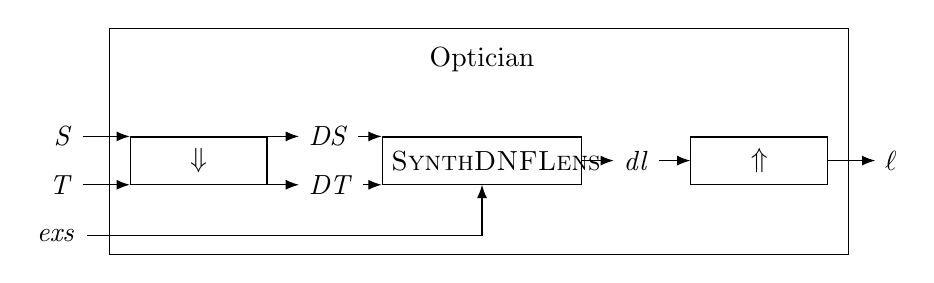
\begin{tikzpicture}[auto,node distance=1.5cm]
    \node[text width=1.5cm,minimum height=.6cm,align=center,draw,rectangle] (todnfregex) {\ToDNFRegex{}};
    
    \node[align=right, anchor=east] (regex1) [left = .6cm of todnfregex.north west]{\Regex{}};
    \node[align=right, anchor=east] (regex2) [left = .6cm of todnfregex.south west]{\RegexAlt{}};
    \node[align=right, anchor=east] (exs) [below = .2cm of regex2]{ \Examples{} };
    
    \node[align=center] (dnfregex1) [right = .4cm of todnfregex.north east]{\DNFRegex{}};
    \node[align=center] (dnfregex2) [right = .4cm of todnfregex.south east]{\DNFRegexAlt{}};

    \node[text width=2.3cm,minimum height=.6cm,align=center,draw,rectangle] [right = 1.45cm of todnfregex.east] (synthdnflens) {\SynthDNFLens{}};
    \node[align=center] [above = .7cm of synthdnflens] (optician) {\Optician{}};
    
    \node[align=center] [right = .4cm of synthdnflens] (dnflens) {\DNFLens{}};
    
    \node[text width=1.5cm,minimum height=.6cm,align=center,draw,rectangle] [right = .4cm of dnflens] (tolens) {\ToLens{}};
    
    \node[align=center] [right = .6cm of tolens] (lens) {\Lens{}};
    
    
    \path[->] (regex1.east) edge (todnfregex.north west);
    \path[->] (regex2.east) edge (todnfregex.south west);
    
    \path[->] (todnfregex.north east) edge (dnfregex1.west);
    \path[->] (todnfregex.south east) edge (dnfregex2.west);
    
    \path[->] (dnfregex1.east) edge (synthdnflens.north west);
    \path[->] (dnfregex2.east) edge (synthdnflens.south west);
    
    \path[->] (synthdnflens) edge (dnflens);
    
    \path[->] (dnflens) edge (tolens);
    
    \path[->] (tolens) edge (lens);
    \draw[->] ($(exs.east)+(-3pt,0)$) -| node(exsedge) {} (synthdnflens);
    \node[fit={($(todnfregex.west)+(-4pt,0)$) ($(tolens.east)+(4pt,0)$) (exsedge) (dnfregex1) (optician) (dnfregex2)},draw] (surrounding) {};
    % Now place a relation (ID=rel1)
    %\node[text width=2cm,align=center,draw, rectangle] (sketch-gen) [right = .75cm of spec] {\TypeProp{}};
    %\node (below-gen) [below=.5cm of sketch-gen] {};
    %\node[text width=2cm,align=center,draw, rectangle] (sketch-compl)
    %     [right = .25cm of sketch-gen] {\RigidSynth{}};
    %\node (below-compl) [below=.5cm of sketch-compl] {};
    %\node[align=center] (lens) [right = .75cm of sketch-compl] {Lens}; 
    %% Draw an edge between rel1 and node1; rel1 and node2
    %\path[->] (spec) edge node (start-alg) {} (sketch-gen);
    %\path[->] (sketch-gen) edge node(middle) {} (sketch-compl);
    %\path[->] (sketch-compl) edge node[near start](success) {\Success{}} (lens);
    %\draw[<-] (sketch-gen.south) -- +(0,-.5) -| node[above left](failure){\Failure{}} (sketch-compl.south);

    %\node (synth-name) [above=.5cm of middle] {\Optician{}};
    %
    %\node[fit=(sketch-gen) (sketch-compl) (start-alg) (synth-name) (failure)
    %(success) ,draw] (surrounding) {};

  \end{tikzpicture}
  \caption{Schematic Diagram for \Optician{}.  Regular expressions, \Regex{} and
    \RegexAlt{}, and examples, \Examples{}, are given as input.
    First, the function \ToDNFRegex{} converts \Regex{} and \RegexAlt{} into
    their respective DNF forms, \DNFRegex{} and \DNFRegexAlt{}.
    Next, \SynthDNFLens{} synthesizes a DNF lens, \DNFLens{}, from \Regex{},
    \RegexAlt{}, and \Examples{}.
    Finally, \ToLens{} converts \DNFLens{} into \Lens{}, a lens in Boomerang
    that is equivalent to \DNFLens{}.}
  \label{fig:schematic-diagram-synthesis}
\end{figure}

Figure~\Cref{fig:schematic-diagram-synthesis} shows a high-level,
schematic diagram for \Optician{}.
First, \Optician{} uses the function \ToDNFRegex{} to convert the input
regular expressions into DNF regular expressions.  Next,
\SynthDNFLens{} performs type-directed synthesis on these DNF regular
expressions and the input examples to synthesize a DNF lens.  Finally, this DNF lens is
converted back into a regular lens with the function \ToLens{}, and returned to the user.


\subsection{Quotient lens synthesis}

Quotient lenses are lenses in which the lens laws are
loosened so that they hold modulo an equivalence relation on the source and
target data respectively; as above, we are concerned with {\em bijective
quotient lenses} which are lenses for which Equation \ref{bijectivelenslaws}
holds modulo equivalence relations $\equiv_S$ and $\equiv_T$ defined on the source
and target data respectively:

\begin{equation}\label{quotientlenslaws}
\ell.\get \; (\ell.\lput \; t) \equiv_T t \text{, and } \ell.\lput \; (\ell.\get
\; s) \equiv_S s
\end{equation}

The inputs to the quotient lens synthesis problem, as in the bijective case,
include source and target regular expressions $S$ and $T$ and a set of example
instances.  The equivalence relations $\equiv_S$ and $\equiv_T$ are also given
as inputs to the synthesis algorithm.  As we describe below, one result of our
work is a language of \textit{quotient regular expressions} that concisely
specifies $S$ and $\equiv_S$ simultaneously.

\section{RESULTS AND DISCUSSION}

Reffing a \Cref{fig:eg}.

\begin{figure}
  a picture is here
  \caption{An example figure}
  \label{fig:eg}
\end{figure}

\section{CONCLUSIONS}

During the course of this project, we have designed, analyzed and implemented algorithms that demonstrate it is possible to synthesize three classes of bidirectional transformations:  (1) pure bijective transformations, (2) bijections modulo equivalences classes and (3) bijections modulo projections.  The synthesis algorithms we have designed take inputs that include a format specification (which includes specification of equivalence classes) and a collection of examples.  As the class of transformations becomes richer, the number of potential programs grows dramatically.  As a result, the corresponding inference algorithm slows and its ability to guess the transformation desired by the user decreases, leading to reduced accuracy.  We found that it was possible to overcome such challenges through new heuristics that use information theory to help guide the search for program transformations.  In addition, we found the use of compositional synthesis, which is the process of breaking down a complex synthesis task into smaller, more mangeable subtasks critical when attempting to scale our prototype system up to be able to handle larger transformation task.

\bibliographystyle{apalike}
\bibliography{local.bib,bcp.bib}

\section{List of Symbols, Abbreviations, and Acronyms}
\begin{tabular}{ll}
  DARPA & Defense Advanced Research Project Agency \\
\end{tabular}

\end{document}

%%% Local Variables:
%%% mode: latex
%%% TeX-master: t
%%% End:
